\chapter{Introduction}

\section{Overview}

Each chapter has its own reference section, which is populated exclusively with the citations from that chapter \cite{Cooper13}.

Figures, like that shown in fig.~\ref{fig:TPBs}, can be inserted in the following manner:

\begin{figure}[H] %The "H" tells latex to put the figure after the previous line and before the next line no matter what.
  \centering
  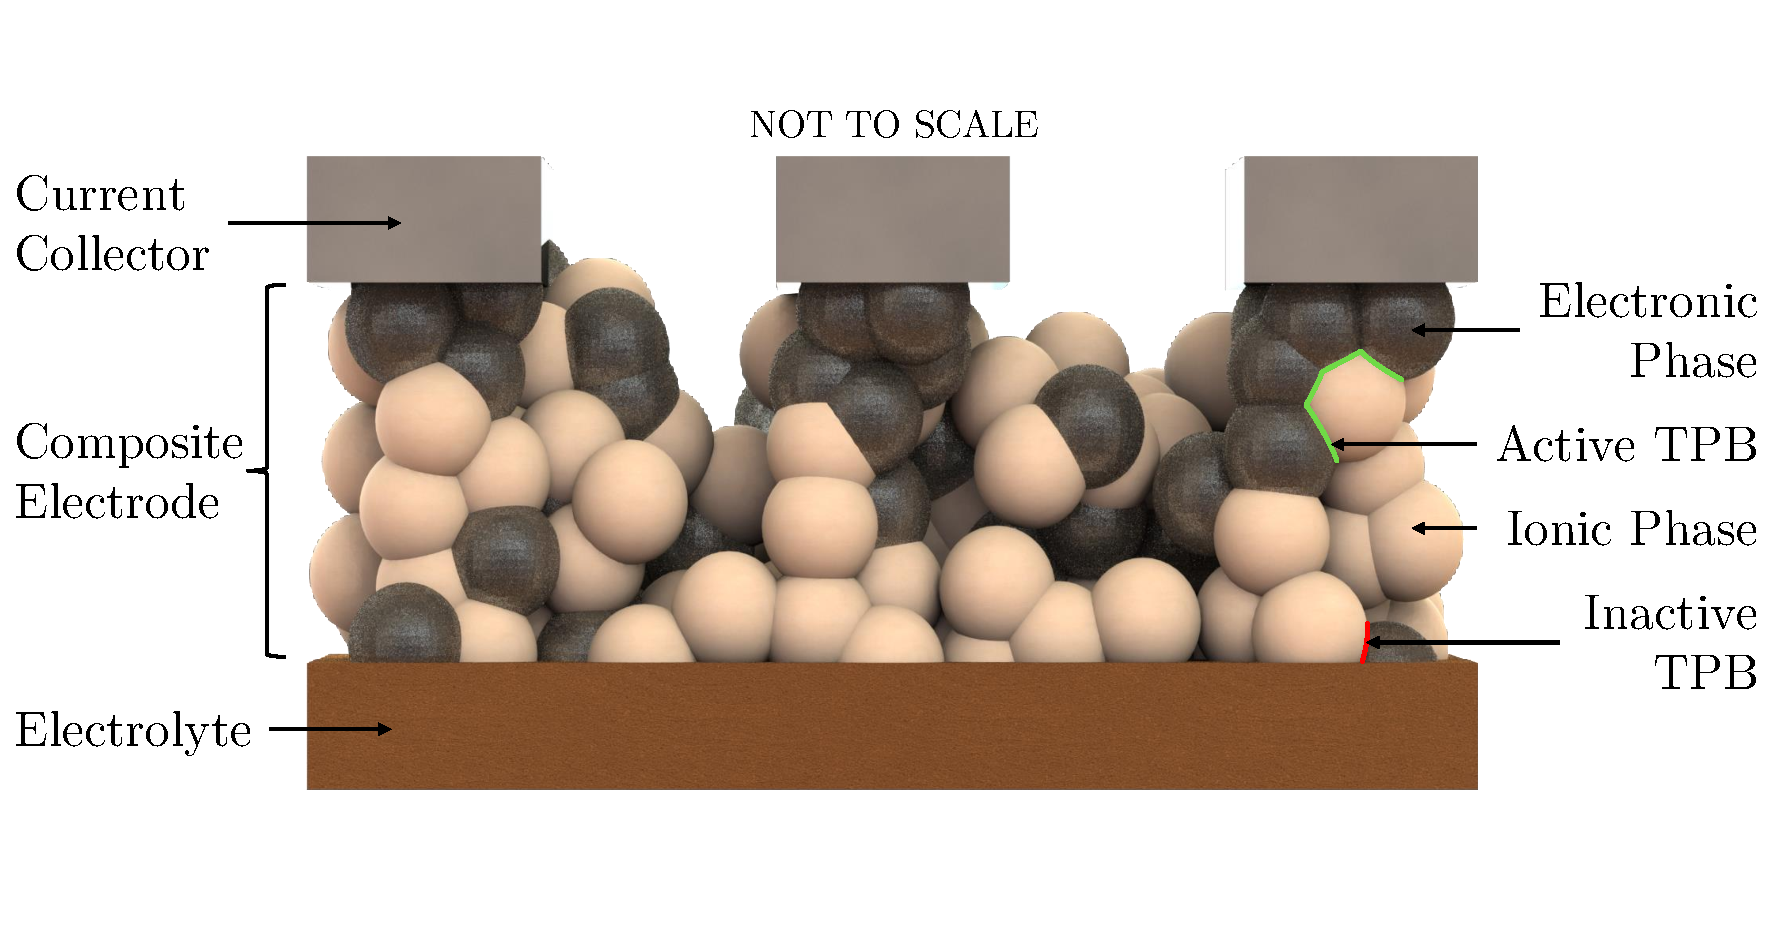
\includegraphics[trim = 0 5mm 0 5mm, clip,width=0.9\textwidth]{C1/Figs/TPBs}
  \caption{Model of a composite porous SOFC electrode, highlighting phase composition and TPB activity.}
  \label{fig:TPBs} 
\end{figure}

Tables look like this follow the form shown in table~\ref{tab:FuelCellTypes}.

\begin{table}[H]
\centering
\caption{Common fuel cell types in order of increasing operating temperature}
\label{tab:FuelCellTypes}
\begin{tabular}{@{}lllll@{}}
\hline
\begin{tabular}[c]{@{}l@{}}Operating\\   Temperature (\celsius)\end{tabular} & Mobile Ion  & Electrolyte                                                           & Name                                                                 & Initialism \\ \hline
50-150                                                                       & OH$^-$      & \begin{tabular}[c]{@{}l@{}}Aqueous\\   alkaline solution\end{tabular} & Alkaline                                                             & AFC        \\
50-200                                                                       & H$^+$       & Ionomer                                                               & \begin{tabular}[c]{@{}l@{}}Proton\\   Exchange Membrane\end{tabular} & PEM        \\
150-250                                                                      & H$^+$       & \begin{tabular}[c]{@{}l@{}}Molten phosphoric\\   acid\end{tabular}    & \begin{tabular}[c]{@{}l@{}}Phosphoric\\   Acid\end{tabular}          & PAFC       \\
600-700                                                                      & CO$_3$$^{2-}$ & \begin{tabular}[c]{@{}l@{}}Molten\\   alkaline carbonate\end{tabular} & \begin{tabular}[c]{@{}l@{}}Molten\\   Carbonate\end{tabular}         & MCFC       \\
500-1000                                                                     & O$^{2-}$    & \begin{tabular}[c]{@{}l@{}}Ceramic\\   Oxide\end{tabular}             & \begin{tabular}[c]{@{}l@{}}Solid\\   Oxide\end{tabular}              & SOFC       \\ \hline
\end{tabular}
\end{table}


Creating the nomenclature requires calling:

\begin{singlespacing}
\begin{lstlisting}[backgroundcolor = \color{lightgray},
                   language = sh,
                   xleftmargin = 2cm,
                   xrightmargin = 2cm,
                   framexleftmargin = 1em]
makeindex %.nlo -s nomencl.ist -o %.nls | txs:///pdflatex | txs:///pdflatex
\end{lstlisting}
\end{singlespacing}

Creating the chapter reference sections requires calling:

\begin{singlespacing}
\begin{lstlisting}[backgroundcolor = \color{lightgray},
                   language = MatLab,
                   xleftmargin = 2cm,
                   xrightmargin = 2cm,
                   framexleftmargin = 1em]
txs:///pdflatex | bibtex C1/chapter1.aux | bibtex C2/chapter2.aux| bibtex C3/chapter3.aux| bibtex C4/chapter4.aux| bibtex C5/chapter5.aux | bibtex C6/chapter6.aux | bibtex CA1/chapterA1.aux | txs:///pdflatex | txs:///pdflatex
\end{lstlisting}
\end{singlespacing}

For everything else, head to the \href{https://en.wikibooks.org/wiki/LaTeX}{\LaTeX Wikibook}.

The \texttt{lipsum} command generates space filling text so that you can more easily see the layout before you've added the content.


\lipsum

\subsection{First Subsection Title}

\lipsum[3]

\section{First Section Title}

\lipsum[4-5]

\pagebreak
%\addcontentsline{toc}{section}{References}
\renewcommand\bibname{{References}}
\bibliography{References}
\bibliographystyle{plain}